\chapter{Problem}
\label{ch:problem}

\section{Problem formulation and research setting}
\label{sec:problem-formulation}

The central problem addressed in this thesis is the classification of Alzheimer's disease (AD)-related clinical groups from peripheral blood gene expression data. More specifically, the thesis focuses on the distinction between subjects diagnosed with AD dementia and subjects diagnosed with mild cognitive impairment (MCI). This choice is deliberate. In much of the blood-transcriptomics literature, the most common benchmark is AD versus cognitively normal controls (CTL). That comparison is useful, but it is also a comparatively easier disease-versus-control setting. The clinically more informative question for this work is whether blood expression profiles contain enough signal to distinguish AD from MCI, two groups that are closer along the clinical continuum of cognitive decline.

This framing follows from the biological and clinical discussion introduced in Chapter~1. AD is no longer understood only as the dementia stage of disease. It is a biological process that can precede clinical dementia by many years, and MCI may represent a symptomatic intermediate stage for some individuals \cite{jack2018nia,albert2011diagnosis}. However, MCI is not equivalent to prodromal AD in every case. It is a heterogeneous clinical category: some subjects may later progress to AD dementia, some may remain stable, and some may have impairment driven by other mechanisms \cite{petersen2004mci}. Therefore, a supervised model trained to separate AD from MCI is not solving a simple healthy-versus-diseased problem. It is learning from two diagnostic labels that are close, noisy, and only partially aligned with the underlying biological disease process.

The labels used in this thesis must therefore be interpreted with caution. They are clinical categories available in public datasets, not direct measurements of amyloid deposition, tau pathology, neuronal injury, or neurodegeneration. In the ideal diagnostic setting, clinical status would be integrated with biomarker evidence. In the present computational setting, the available labels provide a practical supervised learning target. This difference matters because it limits the interpretation of model performance. A classifier that separates AD and MCI may be capturing disease-stage differences, immune and inflammatory alterations, medication-related effects, comorbidities, age-related molecular variation, batch-specific structure, or a mixture of these factors. The thesis therefore treats classification performance as evidence of predictive signal in the available data, not as proof of a clinically deployable diagnostic biomarker.

The biomedical problem is translated into a supervised learning setting. Each subject is represented by a blood gene expression vector
\[
    \mathbf{x}_i \in \mathbb{R}^{p},
\]
where \(p\) denotes the number of retained gene-level expression features after preprocessing. For a dataset of \(n\) subjects, the complete expression matrix is
\[
    \mathbf{X} \in \mathbb{R}^{n \times p}.
\]
For the main task, each subject is assigned a binary label
\[
    y_i \in \{\mathrm{AD}, \mathrm{MCI}\}.
\]
The objective is to learn a predictive function
\[
    f: \mathbb{R}^{p} \rightarrow \{\mathrm{AD}, \mathrm{MCI}\}
\]
that maps each expression profile to its diagnostic label. The same formal structure is used for the reference task AD versus CTL, where the label set is
\[
    y_i \in \{\mathrm{AD}, \mathrm{CTL}\}.
\]

This formulation highlights two dimensions of difficulty. The first is biomedical. The difference between AD and MCI is expected to be subtle because both groups are clinically impaired or disease-adjacent, and MCI itself is biologically heterogeneous. The second is computational. Blood gene expression datasets are high-dimensional and small-sample: thousands of genes are measured for a few hundred subjects. This creates a high-dimensional, low-sample-size setting in which many features may appear discriminative by chance. In such a setting, model evaluation can easily become optimistic if feature selection, scaling, batch correction, or hyperparameter tuning are not handled inside the training procedure.

For this reason, the problem studied in the thesis is not only model selection. It is also a problem of experimental design. A method is useful only if it performs well under a protocol that limits leakage and evaluates generalization to held-out samples. This is especially important because several previous studies in the area report strong results under protocols that are difficult to compare directly. Some focus on AD versus CTL, some use multiclass CN/MCI/AD labels, some study MCI conversion rather than cross-sectional AD/MCI separation, and some apply preprocessing or feature engineering steps before validation. The present thesis therefore defines the task explicitly and uses a common evaluation protocol when comparing reproduced methods.

\section{Datasets}
\label{sec:datasets}

The experimental analysis is based on two public blood gene expression datasets from the Gene Expression Omnibus (GEO): GSE63060 and GSE63061 \cite{barrett2013geo}. Both datasets are associated with the AddNeuroMed study and contain peripheral blood samples from subjects labelled as AD, MCI, or CTL. These two datasets are frequently used in the literature on blood transcriptomics for AD, and for this reason they provide a useful basis for both model development and comparison with previous work.

The use of GSE63060 and GSE63061 is attractive for three reasons. First, they contain all three clinical groups needed to formulate AD/MCI and AD/CTL classification. Second, they are blood-based, which is aligned with the motivation of studying minimally invasive molecular signals. Third, they have been repeatedly used in prior studies, making them a natural reference point for state-of-the-art comparisons.

At the same time, the datasets are not a clean homogeneous benchmark. GSE63060 and GSE63061 were generated in two batches and on two versions of the Illumina HumanHT-12 microarray platform. GSE63060 is associated with the HumanHT-12 V3.0 platform, whereas GSE63061 is associated with the HumanHT-12 V4.0 platform. Therefore, the original probe spaces are not identical, and technical variation may be present even before any biological comparison is considered. In the pipeline used for this thesis, the datasets are harmonized to a common gene-level feature space. After preprocessing and alignment, the binary datasets used in the experiments contain 19,460 gene-level features.

Only samples with one of the target diagnostic labels were retained. Samples with missing, ambiguous, or non-target diagnostic information were excluded from the working cohort. After this filtering step, the full retained dataset contains 711 subjects: 284 AD, 189 MCI, and 238 CTL. The two binary tasks used in the thesis are derived from this retained cohort. The main AD versus MCI task contains 473 samples, while the reference AD versus CTL task contains 522 samples.

\begin{table}[htbp]
\centering
\caption{Working datasets used in this thesis. AD versus MCI is the main task; AD versus CTL is retained as a reference task for comparison with the literature.}
\label{tab:working-datasets}
\begin{tabular}{lccc}
\hline
Dataset & Classes & Samples & Features \\
\hline
Full retained cohort & AD, MCI, CTL & 711 & 19,460 \\
Main task & AD vs MCI & 473 & 19,460 \\
Reference task & AD vs CTL & 522 & 19,460 \\
\hline
\end{tabular}
\end{table}

The class distribution is moderately imbalanced. In the full retained cohort, AD is the largest class, CTL is intermediate, and MCI is the smallest class. In the main AD versus MCI task, the class distribution is 284 AD and 189 MCI. In the AD versus CTL reference task, the distribution is 284 AD and 238 CTL. This imbalance is not extreme, but it is important enough to affect metric choice. A model that predicts the majority class more reliably may obtain acceptable accuracy while still performing poorly on the minority class. This is one of the reasons why macro-F1 is used throughout the thesis.

\begin{table}[htbp]
\centering
\caption{Class distribution in the retained datasets.}
\label{tab:class-distribution}
\begin{tabular}{lccc}
\hline
Setting & AD & MCI & CTL \\
\hline
Full retained cohort & 284 & 189 & 238 \\
AD vs MCI & 284 & 189 & -- \\
AD vs CTL & 284 & -- & 238 \\
\hline
\end{tabular}
\end{table}

The available metadata include age, gender, ethnicity, clinical status, GEO accession, and dataset origin. These variables are important for describing the cohort and for identifying possible confounding factors. However, the thesis does not treat demographic metadata as the central predictive input. The main experimental question is whether transcriptomic profiles alone provide useful signal. Metadata are therefore discussed only insofar as they affect interpretation: age, sex, ethnicity, and dataset origin can all influence blood gene expression, and therefore they may contribute to apparent classification signal if not handled carefully.

The dataset origin variable is especially relevant because it identifies whether a sample comes from GSE63060 or GSE63061. This variable is not a biological label, but it can be correlated with technical effects. A classifier that learns to separate datasets rather than disease states would be misleading. For this reason, the evaluation protocol must make the batch structure visible. Internal random splits can be useful, but they are not sufficient on their own. Batch-holdout or cross-dataset tests are more informative because they evaluate whether a learned pattern survives a shift between dataset batches.

In summary, GSE63060 and GSE63061 provide a suitable but challenging data source for this thesis. They are suitable because they contain blood expression profiles for AD, MCI, and CTL subjects and because they are widely used in the literature. They are challenging because they combine high dimensionality, moderate class imbalance, MCI heterogeneity, and technical batch structure. The dataset should therefore be treated as an experimental benchmark for predictive modelling, not as a complete clinical validation cohort.

\section{Classification tasks and metrics}
\label{sec:classification-tasks}

The thesis distinguishes between the main task and the reference task. The main task is AD versus MCI:
\[
    \mathcal{T}_{\mathrm{main}} = \mathrm{AD} \; \mathrm{vs.} \; \mathrm{MCI}.
\]
This is the primary benchmark for the work. It is the most relevant task for evaluating whether blood transcriptomics can provide information near the transition from mild impairment to dementia. It is also the task where performance is expected to be lower, because the two groups are closer than AD and CTL.

The reference task is AD versus CTL:
\[
    \mathcal{T}_{\mathrm{ref}} = \mathrm{AD} \; \mathrm{vs.} \; \mathrm{CTL}.
\]
This task is included because it is the dominant setting in previous blood-transcriptomic AD studies. It allows the reproduced methods and the proposed model to be compared against the type of benchmark most often reported in the literature. However, it is not used as the main evidence for the thesis claim. A method that performs well on AD versus CTL may still have limited value for early-stage discrimination if it cannot separate AD from MCI.

The thesis does not treat multiclass CTL versus MCI versus AD classification as the central task at this stage. Multiclass classification is clinically interesting, but it mixes several decision boundaries into a single score. A model may perform well on the easier AD/CTL contrast while performing poorly on MCI. For the present thesis, it is more informative to isolate the pairwise tasks and compare AD/MCI directly with AD/CTL. This makes the difficulty difference explicit and avoids hiding MCI errors inside a single multiclass aggregate.

Three primary metrics are used: accuracy, macro-F1, and ROC-AUC. Accuracy is the most intuitive metric and measures the proportion of correct predictions:
\[
    \mathrm{Accuracy} =
    \frac{\mathrm{correct\ predictions}}{\mathrm{total\ predictions}}.
\]
Accuracy is useful because it is easy to interpret and commonly reported in the literature. However, it can be misleading when classes are imbalanced or when one class is systematically easier than the other. For example, in AD versus MCI, a classifier could improve accuracy by favoring AD because AD is the larger class. This would not necessarily indicate a clinically useful model.

Macro-F1 is therefore used as the main class-balanced summary metric. For each class \(k\), precision and recall are defined as
\[
    \mathrm{Precision}_k =
    \frac{\mathrm{TP}_k}{\mathrm{TP}_k+\mathrm{FP}_k},
\]
and
\[
    \mathrm{Recall}_k =
    \frac{\mathrm{TP}_k}{\mathrm{TP}_k+\mathrm{FN}_k}.
\]
The class-specific F1-score is the harmonic mean of precision and recall:
\[
    F1_k =
    2 \cdot
    \frac{\mathrm{Precision}_k \cdot \mathrm{Recall}_k}
    {\mathrm{Precision}_k + \mathrm{Recall}_k}.
\]
Macro-F1 averages the F1-scores across classes:
\[
    \mathrm{Macro\mbox{-}F1} =
    \frac{1}{K}\sum_{k=1}^{K} F1_k.
\]
In the binary tasks considered here, \(K=2\). Macro-F1 gives equal weight to both classes, regardless of their sample size. This makes it more appropriate than accuracy when the objective is to avoid a model that performs well only on the majority class.

ROC-AUC evaluates the ability of a classifier to rank positive samples above negative samples across possible thresholds. It is useful because it uses the model scores before thresholding and is widely reported in biomedical classification. In this thesis, ROC-AUC is interpreted together with accuracy and macro-F1. A model can have a reasonable ROC-AUC while still producing poor discrete classifications at a chosen threshold. Conversely, a model can have acceptable accuracy but weak ranking ability. Reporting all three metrics gives a more complete picture of performance.

The interpretation of the positive class is task-dependent. In AD versus MCI, AD is treated as the positive class in the binary formulation. In AD versus CTL, AD is also treated as the positive class. This convention is consistent with the disease-detection framing. However, the thesis is not only interested in detecting AD. In AD versus MCI, the MCI class is equally important because it represents the clinically ambiguous group. This is another reason for prioritizing macro-F1.

The task and metric choices are therefore aligned with the research question. AD versus MCI is the main task because it addresses the more difficult and clinically relevant boundary. AD versus CTL is the reference task because it connects the work to the dominant literature. Accuracy, macro-F1, and ROC-AUC are reported together because no single metric is sufficient in a high-dimensional and moderately imbalanced biomedical classification problem.

\section{Main challenges}
\label{sec:main-challenges}

The first challenge is the weak visual separability of the expression matrix. If AD and MCI were strongly separated by a small number of expression patterns, one might expect unsupervised visualizations to reveal clear class-specific blocks. This is not what is observed. Figure~\ref{fig:ch2-heatmap} shows the top 1000 genes selected only by variance in the AD versus MCI dataset. Samples are kept in their processed order and no clustering is applied to the sample axis. The label strip shows the clinical class, while the heatmap shows gene-wise standardized expression values. The resulting pattern is dense and heterogeneous. There is no simple block structure that visually separates AD from MCI.

\begin{figure}[htbp]
\centering
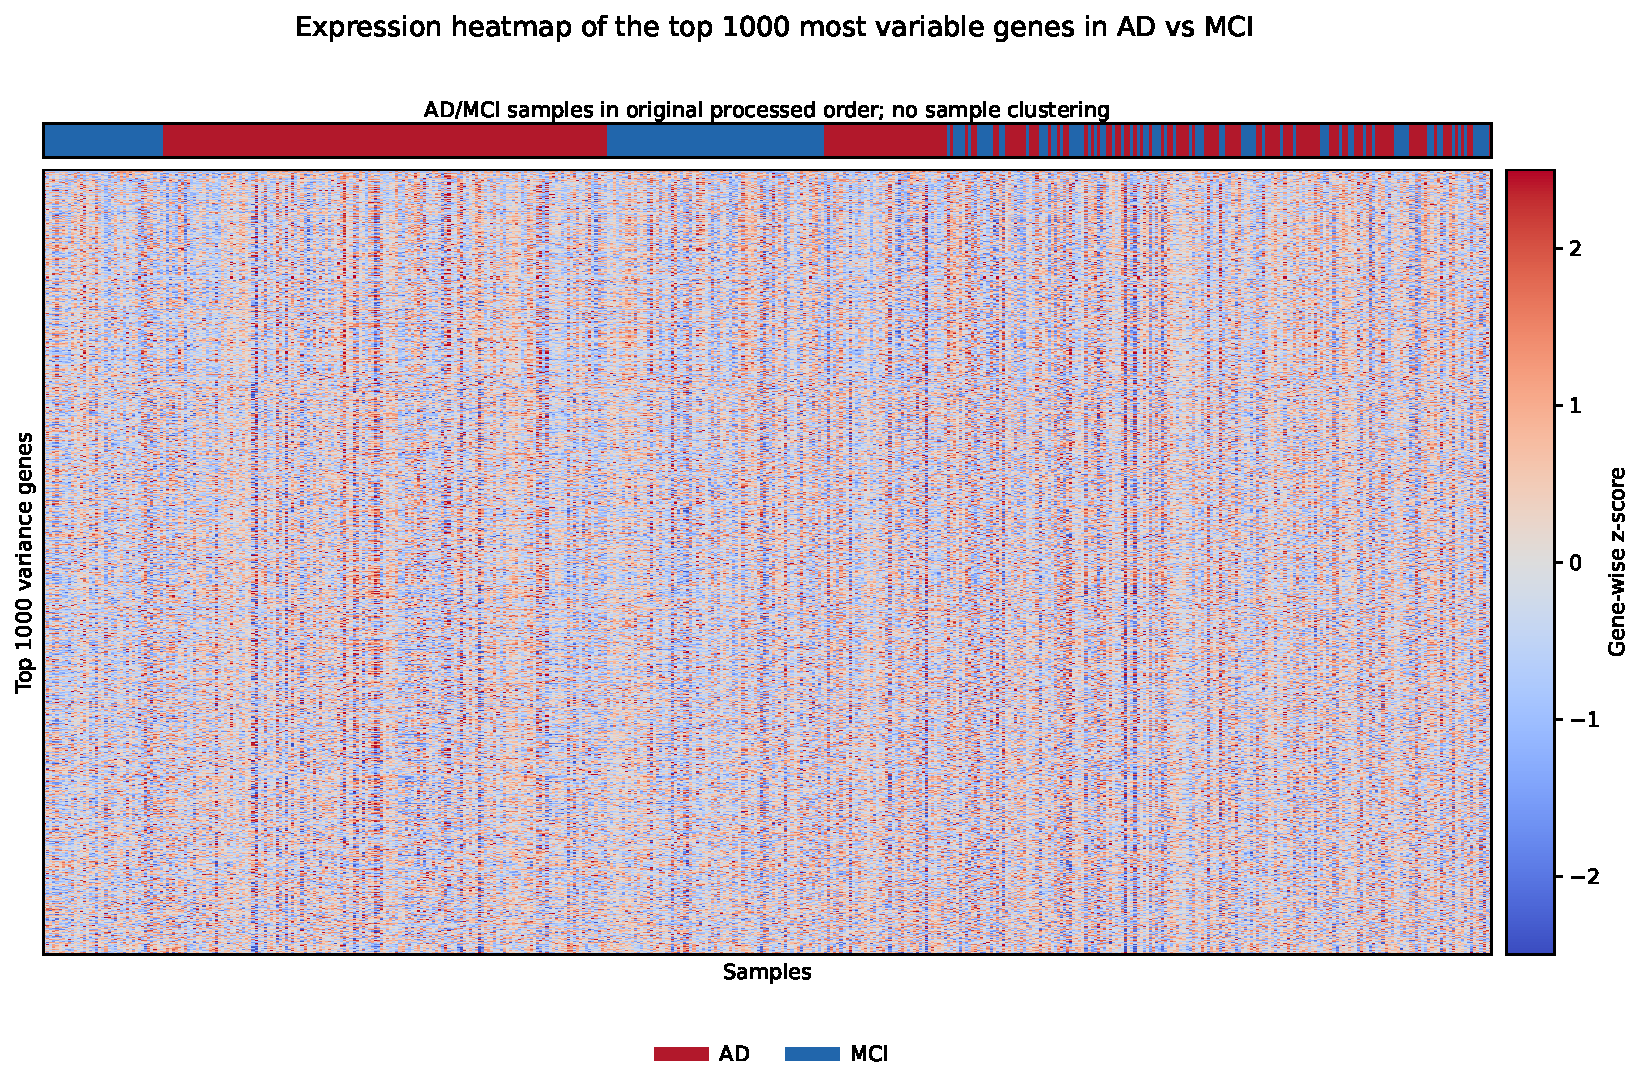
\includegraphics[width=\textwidth]{figures/ch2_heatmap_top1000_variance_ad_mci.pdf}
\caption{Heatmap of the 1000 most variable genes in the AD versus MCI dataset. Expression values are gene-wise standardized and clipped for visualization. Samples are not clustered; the top annotation indicates the clinical label. The absence of clear block structure illustrates the limited separability of AD and MCI from expression values alone.}
\label{fig:ch2-heatmap}
\end{figure}

This figure is descriptive rather than inferential. It does not prove that classification is impossible, and it does not replace a supervised benchmark. Its purpose is to show the geometry of the raw problem. The expression matrix does not provide an obvious visual separation between the two classes. Any useful model must therefore learn subtle distributed patterns rather than exploit a clear class partition visible in the top-variance genes.

The second challenge is class overlap in low-dimensional expression space. Figure~\ref{fig:ch2-pca} shows two-dimensional PCA projections for AD versus MCI and AD versus CTL, again using top-variance expression features. PCA is unsupervised and is not optimized for classification. Nevertheless, it is useful as a diagnostic visualization of global variance structure. In both panels, the classes overlap substantially. The AD versus CTL panel shows a slightly more interpretable trend, while the AD versus MCI panel is highly mixed. This supports the central premise of the thesis: AD versus CTL is a useful reference, but AD versus MCI is the main difficult task.

\begin{figure}[htbp]
\centering
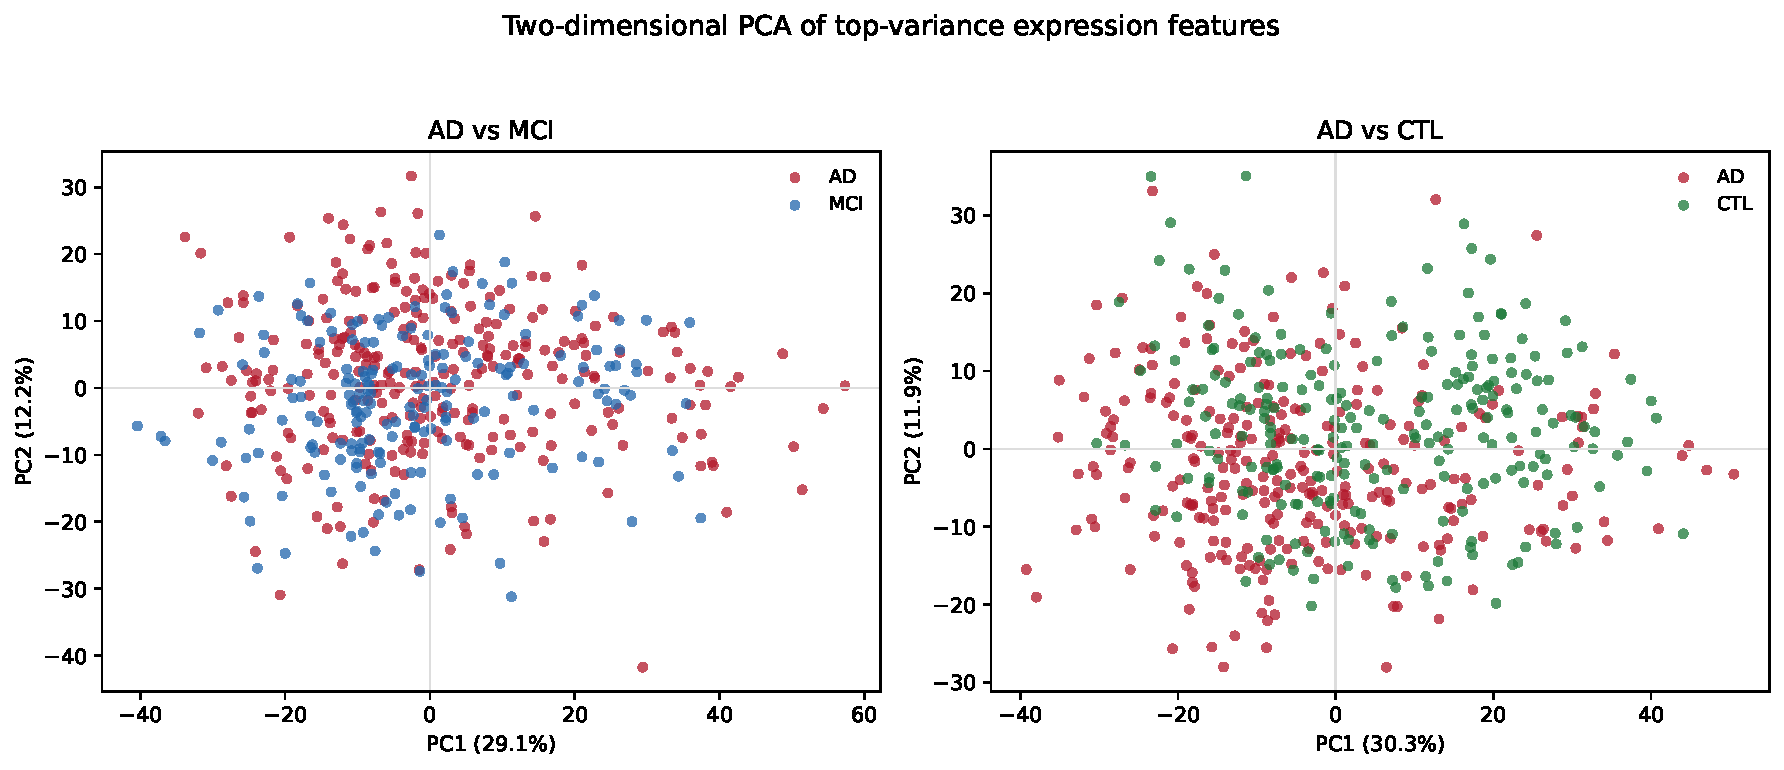
\includegraphics[width=\textwidth]{figures/ch2_pca_ad_mci_ad_ctl.pdf}
\caption{Two-dimensional PCA projections of top-variance expression features for AD versus MCI and AD versus CTL. The projections are unsupervised and are used only to visualize the geometry of the expression space. The strong overlap, especially for AD versus MCI, motivates careful validation and class-balanced metrics.}
\label{fig:ch2-pca}
\end{figure}

The third challenge is high dimensionality. Each subject is described by 19,460 expression features, while the number of samples is in the order of hundreds. This creates many opportunities for spurious associations. Some genes may appear strongly associated with the label only because of the specific split, the batch composition, or random sampling variation. This problem affects both classical machine learning and deep learning. Classical models may overfit through unstable feature selection. Neural models may overfit through excessive capacity relative to the sample size. Regularization and careful validation are therefore necessary, but they are not sufficient unless the entire pipeline is split-aware.

The fourth challenge is feature selection. Reducing the feature space can improve stability and make models easier to train, but feature selection is also one of the most common sources of leakage in transcriptomic studies. If genes are selected using the full dataset before the train-test split, the test labels influence the training pipeline. Even if the final classifier does not directly see the test labels, the feature space has already been optimized using information from the test distribution. This is especially damaging in high-dimensional data, where the number of possible feature subsets is enormous. In this thesis, feature selection is treated as part of the training procedure and must not be fitted on held-out test samples.

The fifth challenge is batch structure. GSE63060 and GSE63061 are related, but they are not technically identical. Batch correction methods such as ComBat can reduce unwanted technical variation \cite{johnson2007combat}, but they can also introduce leakage if fitted on the full dataset before validation. The same issue applies to scaling and normalization parameters. If test samples contribute to the estimation of preprocessing parameters, the evaluation becomes optimistic. Therefore, batch effects are not only a biological or technical nuisance; they are also a validation problem.

The sixth challenge is the biological heterogeneity of MCI. The MCI label includes subjects who may be at different points along the AD continuum and subjects whose impairment may not be AD-related. This means that the MCI class may overlap with both CTL and AD at the molecular level. A model that confuses some MCI subjects with AD may be detecting real disease-stage proximity, or it may simply be failing to separate noisy labels. Without longitudinal follow-up and biomarker confirmation, these possibilities cannot be fully disentangled. This limitation must be kept in mind when interpreting AD/MCI errors.

The final challenge is generalization. A model trained on GSE63060 and GSE63061 may perform well on one split and still fail on a different cohort, platform, or population. Blood gene expression is influenced by age, sex, immune state, medication, sample handling, and many other factors. The thesis therefore avoids presenting model performance as a definitive clinical diagnostic result. Instead, performance is interpreted as evidence about the predictive value and limitations of blood transcriptomic profiles under a controlled experimental protocol. This conservative interpretation is necessary because the main task, AD versus MCI, sits at the intersection of subtle biology, imperfect clinical labels, and high-dimensional machine learning.
